\section{Cost of Transformative Write IO}

In this section, we show the performance implications of transformative IO by
examining the metadata request load incurred by PLFS. We use CephFS, the
POSIX-compliant file system that uses Ceph's RADOS object
store~\cite{weil:osdi2006-ceph}, as the underlying file system.  This analysis
focuses on the file system metadata RPCs between the client and metadata server
and does not include the RPCs needed to write and read actual data.  We use two
workloads: processes writing to variable offsets in a single PLFS file
(microbenchmark) and processes replaying a PLFS trace\footnote{Traces found
here:
\href{https://web.archive.org/web/20140419194914/http://institutes.lanl.gov/plfs/maps/}{here}}
(macrobenchmark). 

CephFS uses a cluster of metadata servers to service file system metadata
requests~\cite{weil:sc2004-dyn-metadata} and to characterize the workload, we
instrumented the metadata server to track (1) the number of each request type
\footnote{This code was merged into the Ceph project.} and (2) the heat of each
directory.  We could have used the client with FUSE debugging turned on but
that would show all issued requests regardless of whether they were sent to the
metadata server. In CephFS the protocols for caching may reduce the number of
\texttt{lookup} requests that hit the metadata server and we did not want to
count those requests as work down by the metadata server.


\subsection{Overhead of Metadata Writes}
When PLFS maps a logical file to many physical files, it deterministically
creates the file system namespace in the backend file system.  For \(n\)
processes on \(m\) servers:

\begin{itemize}
  \item create directories: \(m \times \texttt{mkdir()}\)
  \item create files: \(2n \times \texttt{create()} [+ 2n \times \texttt{lookup()}]\)
  \item files/directory: \(n/m\)
\end{itemize}

% How does PLFS create namespaces
The number of directories is dependent on the number of PLFS servers. When a file is created in
a PLFS mount, a directory called a container is created in the underlying file
system. Inside the container, directories are created per server resulting in
\(m\) requests. The number of files is dependendent on the number of PLFS
processes. Processes write data and index files to the directory assigned to
their server. The number of requests, which can range from \(2n\) to \(4n\), is
a function of files per directory.  If each server only has one process, then
the number of file create requests will be \(2n\) because each process can
cache the directory inode and create files in one request. With multiple
processes per server, clients write to the same directory and the number of
requests doubles because processes cannot cache the directory inode.

\subsubsection{Microbenchmark}
TODO: multiple processes per node
TODO: verify path traversal
\begin{figure}[tb]
\centering
  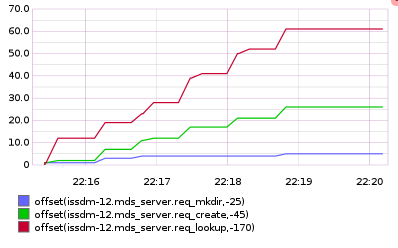
\includegraphics[width=90mm]{figures/prob_reqs.png} 
  \caption{The requests scale linearly with the number of clients.
  \texttt{lookup()} requests dominate because clients share the root and must do
  path traversal.
  }\label{fig:arch}
\end{figure}

%
\subsubsection{Macrobenchmark}

\subsection{Overhead of Reads}

% How does PLFS read the namespace
Transforming write IO in this way has space and read overheads. In PLFS, this
is a problem because index files need to be coalesced on reads.  Patterned
PLFS~\cite{he:hpdc13-plfs-patterns} reduces the space overheads by storing
formulas, instead of index files, to represent write behavior. Diddlings
~\cite{grider:pc17-diddlings} transfers index files after each write to absorb
the transfer overheads up front. While these approaches help alleviate read
overheads, they do not reduce the file system metadata load, which is the real
problem. Reading the index file still requires a file system metadata
operation.

\begin{itemize}
  \item read file: \(2n \times \texttt{open()}\) 
\end{itemize}

\subsubsection{Microbenchmark}
\subsubsection{Macrobenchmark}
